\documentclass{standalone}
\usepackage[utf8]{inputenc}
\usepackage{pgfplots}
\DeclareUnicodeCharacter{2212}{−}
\usepgfplotslibrary{groupplots,dateplot}
\usetikzlibrary{patterns,shapes.arrows}
\pgfplotsset{compat=newest}
\begin{document}
% This file was created with tikzplotlib v0.10.1.
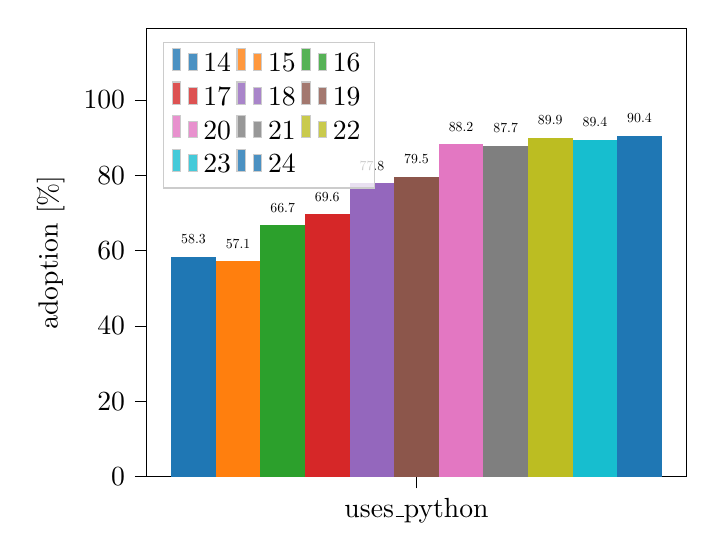
\begin{tikzpicture}

\definecolor{crimson2143940}{RGB}{214,39,40}
\definecolor{darkgray176}{RGB}{176,176,176}
\definecolor{darkorange25512714}{RGB}{255,127,14}
\definecolor{darkturquoise23190207}{RGB}{23,190,207}
\definecolor{forestgreen4416044}{RGB}{44,160,44}
\definecolor{goldenrod18818934}{RGB}{188,189,34}
\definecolor{gray127}{RGB}{127,127,127}
\definecolor{lightgray204}{RGB}{204,204,204}
\definecolor{mediumpurple148103189}{RGB}{148,103,189}
\definecolor{orchid227119194}{RGB}{227,119,194}
\definecolor{sienna1408675}{RGB}{140,86,75}
\definecolor{steelblue31119180}{RGB}{31,119,180}

\begin{axis}[
legend cell align={left},
legend columns=3,
legend style={
  fill opacity=0.8,
  draw opacity=1,
  text opacity=1,
  at={(0.03,0.97)},
  anchor=north west,
  draw=lightgray204
},
tick align=outside,
tick pos=left,
x grid style={darkgray176},
xmin=-0.404, xmax=0.564,
xtick style={color=black},
xtick={0.08},
xticklabels={uses\_python},
y grid style={darkgray176},
ylabel={adoption [\%]},
ymin=0, ymax=119,
ytick style={color=black}
]
\draw[draw=none,fill=steelblue31119180] (axis cs:-0.36,0) rectangle (axis cs:-0.28,58.3);
\addlegendimage{ybar,ybar legend,draw=none,fill=steelblue31119180}
\addlegendentry{14}

\draw[draw=none,fill=darkorange25512714] (axis cs:-0.28,0) rectangle (axis cs:-0.2,57.1);
\addlegendimage{ybar,ybar legend,draw=none,fill=darkorange25512714}
\addlegendentry{15}

\draw[draw=none,fill=forestgreen4416044] (axis cs:-0.2,0) rectangle (axis cs:-0.12,66.7);
\addlegendimage{ybar,ybar legend,draw=none,fill=forestgreen4416044}
\addlegendentry{16}

\draw[draw=none,fill=crimson2143940] (axis cs:-0.12,0) rectangle (axis cs:-0.04,69.6);
\addlegendimage{ybar,ybar legend,draw=none,fill=crimson2143940}
\addlegendentry{17}

\draw[draw=none,fill=mediumpurple148103189] (axis cs:-0.04,0) rectangle (axis cs:0.04,77.8);
\addlegendimage{ybar,ybar legend,draw=none,fill=mediumpurple148103189}
\addlegendentry{18}

\draw[draw=none,fill=sienna1408675] (axis cs:0.04,0) rectangle (axis cs:0.12,79.5);
\addlegendimage{ybar,ybar legend,draw=none,fill=sienna1408675}
\addlegendentry{19}

\draw[draw=none,fill=orchid227119194] (axis cs:0.12,0) rectangle (axis cs:0.2,88.2);
\addlegendimage{ybar,ybar legend,draw=none,fill=orchid227119194}
\addlegendentry{20}

\draw[draw=none,fill=gray127] (axis cs:0.2,0) rectangle (axis cs:0.28,87.7);
\addlegendimage{ybar,ybar legend,draw=none,fill=gray127}
\addlegendentry{21}

\draw[draw=none,fill=goldenrod18818934] (axis cs:0.28,0) rectangle (axis cs:0.36,89.9);
\addlegendimage{ybar,ybar legend,draw=none,fill=goldenrod18818934}
\addlegendentry{22}

\draw[draw=none,fill=darkturquoise23190207] (axis cs:0.36,0) rectangle (axis cs:0.44,89.4);
\addlegendimage{ybar,ybar legend,draw=none,fill=darkturquoise23190207}
\addlegendentry{23}

\draw[draw=none,fill=steelblue31119180] (axis cs:0.44,0) rectangle (axis cs:0.52,90.4);
\addlegendimage{ybar,ybar legend,draw=none,fill=steelblue31119180}
\addlegendentry{24}

\draw (axis cs:-0.32,58.3) ++(0pt,3pt) node[
  scale=0.5,
  anchor=south,
  text=black,
  rotate=0.0
]{58.3};
\draw (axis cs:-0.24,57.1) ++(0pt,3pt) node[
  scale=0.5,
  anchor=south,
  text=black,
  rotate=0.0
]{57.1};
\draw (axis cs:-0.16,66.7) ++(0pt,3pt) node[
  scale=0.5,
  anchor=south,
  text=black,
  rotate=0.0
]{66.7};
\draw (axis cs:-0.08,69.6) ++(0pt,3pt) node[
  scale=0.5,
  anchor=south,
  text=black,
  rotate=0.0
]{69.6};
\draw (axis cs:0,77.8) ++(0pt,3pt) node[
  scale=0.5,
  anchor=south,
  text=black,
  rotate=0.0
]{77.8};
\draw (axis cs:0.08,79.5) ++(0pt,3pt) node[
  scale=0.5,
  anchor=south,
  text=black,
  rotate=0.0
]{79.5};
\draw (axis cs:0.16,88.2) ++(0pt,3pt) node[
  scale=0.5,
  anchor=south,
  text=black,
  rotate=0.0
]{88.2};
\draw (axis cs:0.24,87.7) ++(0pt,3pt) node[
  scale=0.5,
  anchor=south,
  text=black,
  rotate=0.0
]{87.7};
\draw (axis cs:0.32,89.9) ++(0pt,3pt) node[
  scale=0.5,
  anchor=south,
  text=black,
  rotate=0.0
]{89.9};
\draw (axis cs:0.4,89.4) ++(0pt,3pt) node[
  scale=0.5,
  anchor=south,
  text=black,
  rotate=0.0
]{89.4};
\draw (axis cs:0.48,90.4) ++(0pt,3pt) node[
  scale=0.5,
  anchor=south,
  text=black,
  rotate=0.0
]{90.4};
\end{axis}

\end{tikzpicture}

\end{document}